\chapter{Analyse du Système}

Cette section formalise l'analyse conceptuelle du module de facturation (\textit{Billing Service}) de l'ERP ComOps. Elle définit la problématique d'ingénierie et détaille la modélisation conceptuelle à travers différents diagrammes UML.

\section{Problématique}
La conception initiale du Billing Service souffrait d'un défaut majeur d'architecture : la réplication locale des entités de tiers (clients et fournisseurs) au sein de sa base de données propre. Cette duplication présentait plusieurs inconvénients majeurs en ingénierie logicielle :
\begin{itemize}
    \item \textbf{Désynchronisation des données} : Toute mise à jour effectuée sur la fiche d'un tiers dans le noyau central (\textit{Kernel}) n'était pas propagée instantanément au module Billing, conduisant à des factures contenant des données erronées ou obsolètes (adresses de facturation incorrectes, mauvais numéros de TVA intracommunautaire).
    \item \textbf{Violation du principe de responsabilité unique (SRP)} : Le Billing Service devait intégrer du code et des modèles pour gérer le cycle de vie des clients, augmentant inutilement sa complexité et son coût de maintenance.
    \item \textbf{Couplage fort de base de données} : La dépendance vis-à-vis de tables physiques dupliquées empêchait toute autonomie de déploiement et d'évolution du schéma de données.
\end{itemize}
L'objectif de cette analyse est de concevoir une intégration dynamique non bloquante où le Kernel est l'unique source de vérité, tout en préservant l'isolation multi-tenant et la performance réactive du système.

\section{Modélisation Conceptuelle}
La modélisation conceptuelle permet d'établir une vue d'ensemble du système, de ses limites, de sa structure modulaire, de son modèle de domaine et de la dynamique de ses états, indépendamment des frameworks techniques d'implémentation.

\subsection{Diagramme de Contexte}
Le diagramme de contexte définit les frontières du système de facturation et ses interactions avec l'environnement externe de l'ERP ComOps.

\begin{figure}[htbp]
\centering
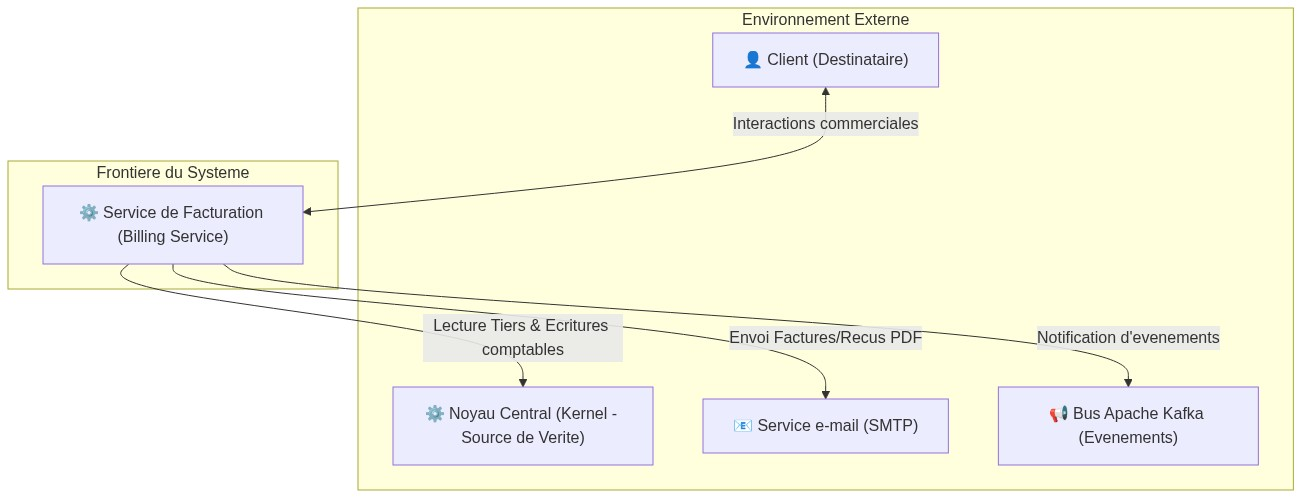
\includegraphics[width=0.9\textwidth]{images/context_diagram.png}
\caption{Diagramme de Contexte du Billing Service .}
\label{fig:context_diagram}
\end{figure}

Le diagramme (Figure \ref{fig:context_diagram}) montre que le Billing Service agit comme un composant pivot qui interagit avec le client final, s'appuie sur le Kernel pour la cohérence des tiers et de la comptabilité générale, et notifie les autres modules via Kafka et le service de messagerie SMTP.

\subsection{Diagramme de Packages}
Le diagramme de packages présente la structure d'organisation modulaire du Billing Service selon les principes de conception de l'architecture hexagonale.

\begin{figure}[htbp]
\centering
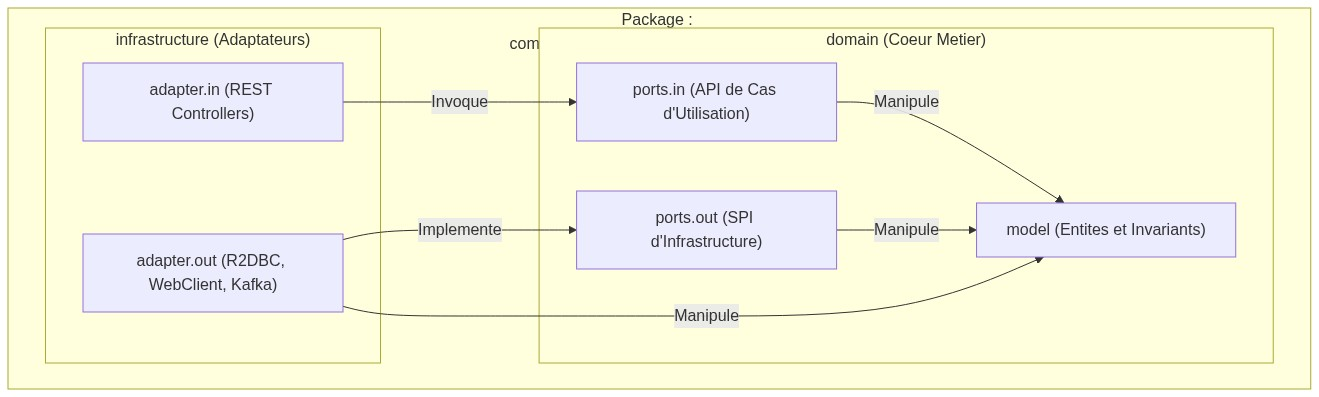
\includegraphics[width=0.9\textwidth]{images/package_diagram.png}
\caption{Diagramme de Packages de l'Architecture Hexagonale .}
\label{fig:package_diagram}
\end{figure}

Le diagramme (Figure \ref{fig:package_diagram}) illustre la règle de dépendance : les packages de l'infrastructure dépendent du package du domaine central. Les détails d'infrastructure implémentent les ports sortants (\textit{SPI}) ou appellent les ports entrants (\textit{API}), garantissant que la logique métier reste isolée des frameworks techniques.

\subsection{Diagramme de Classes d'Analyse}
Le diagramme de classes d'analyse modélise la structure logique du domaine fonctionnel, en décrivant les entités métiers, les interfaces de ports de communication et le service de contrôle.

\begin{figure}[htbp]
\centering
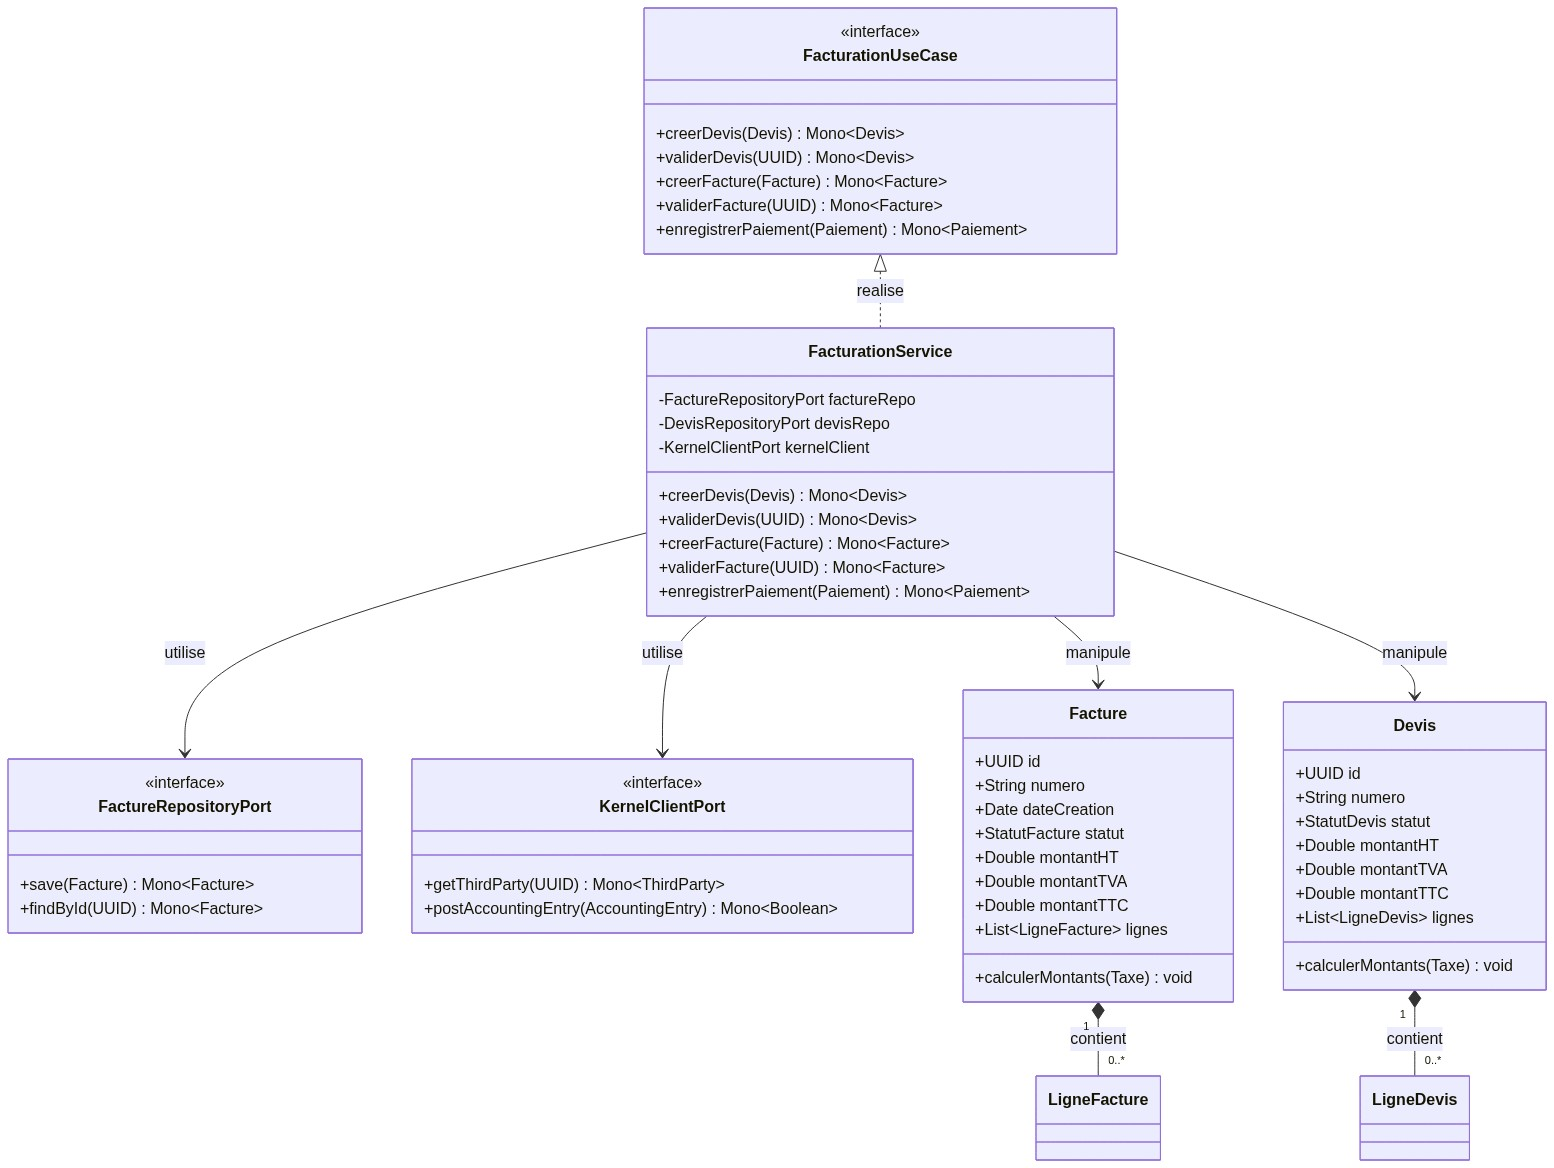
\includegraphics[width=0.9\textwidth]{images/analysis_class_diagram.png}
\caption{Diagramme de Classes d'Analyse du Domaine Métier .}
\label{fig:analysis_class_diagram}
\end{figure}

Le diagramme (Figure \ref{fig:analysis_class_diagram}) représente les entités et ports du domaine. Le domaine métier ne contient aucune classe d'infrastructure. Le service de contrôle (\texttt{FacturationService}) coordonne l'exécution en utilisant des interfaces abstraites de ports pour interagir avec la persistance ou les API externes.

\subsection{Diagramme de Cas d'Utilisation}
Le diagramme de cas d'utilisation illustre les rôles des différents acteurs vis-à-vis du système, délimitant l'accès aux fonctionnalités métiers.

\begin{figure}[htbp]
\centering
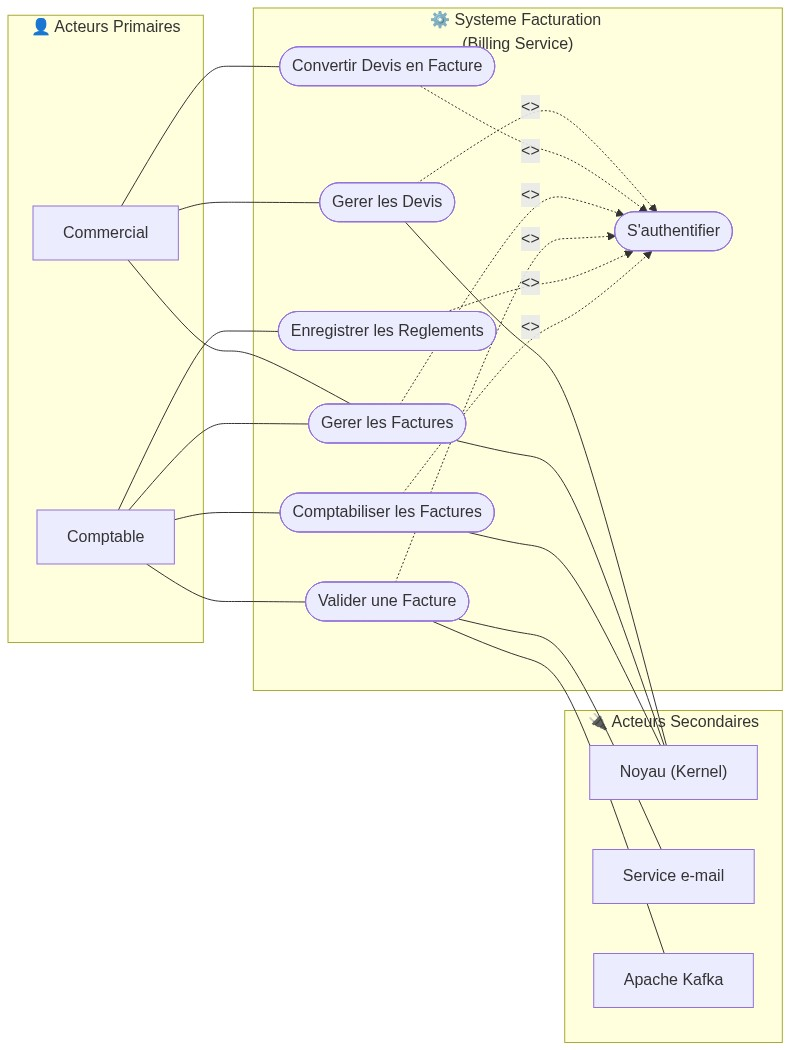
\includegraphics[width=0.9\textwidth]{images/use_case.png}
\caption{Diagramme de Cas d'Utilisation du Module Billing .}
\label{fig:use_case}
\end{figure}

Le diagramme (Figure \ref{fig:use_case}) formalise les interactions : l'agent commercial pilote la saisie commerciale, le comptable gère la partie comptable et financière, et l'accès est conditionné par une authentification systématique.

\subsection{Diagramme d'États-Transitions}
Le cycle de vie fonctionnel des documents de facturation est décrit par la machine à états finis régissant l'évolution d'une facture.

\begin{figure}[htbp]
\centering
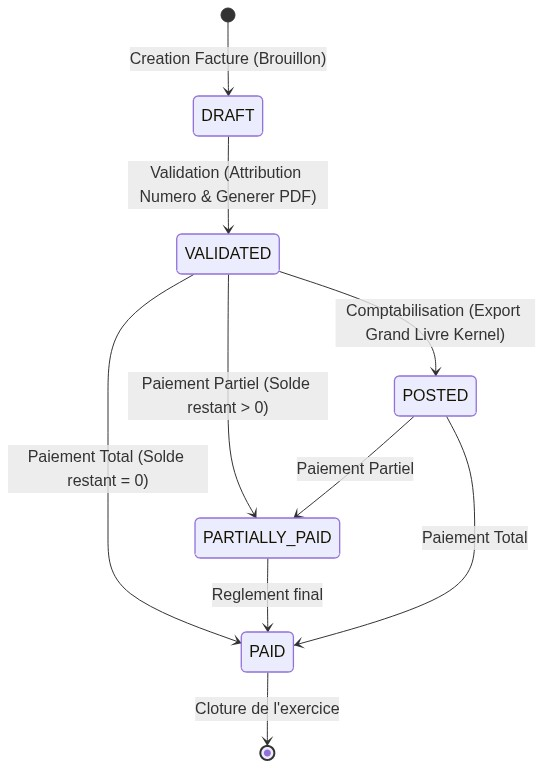
\includegraphics[width=0.9\textwidth]{images/state_diagram.png}
\caption{Diagramme d'État-Transition UML du Cycle de Vie d'une Facture .}
\label{fig:state_diagram}
\end{figure}

Le diagramme (Figure \ref{fig:state_diagram}) structure les changements d'états d'une facture. Les transitions sont guidées par les événements métiers : validation, paiement (partiel ou total), et comptabilisation dans le grand livre du Kernel.
